\def\rescaledPrismTikz
{
\begin{figure}[!h]
	\centering
	\subfloat
	{	
		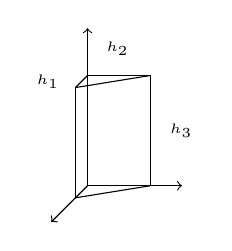
\begin{tikzpicture}[scale=.4]
		\label{rescaled_prism}		
		  \draw[xshift = 6cm, ->] (0, 0) -- (0, 0, 3);	
		  \draw[xshift = 6cm, ->] (0, 0) -- (3,0);
		  \draw[xshift = 6cm, ->] (0, 0) --  (0, 5, 0);
		  \draw[xshift = 6cm] (0, 0, 1) -- (2, 0, 0); 
		  \draw[xshift = 6cm] (0, 3.5, 1) -- (2, 3.5, 0); 
		  \draw[xshift = 6cm] (2, 0, 0) -- node[label={right:$_{_{h_3}}$}] { } (2, 3.5, 0);
		  \draw[xshift = 6cm] (0, 0, 1) -- (0, 3.5, 1); 
		  \draw[xshift = 6cm] (0,3.5,1) -- node[label={left:$_{_{h_1}}$}] { }  (0,3.5,0) ;
		  \draw[xshift = 6cm] (0,3.5,0) -- node[label={above:$_{_{h_2}}$}] { } (2,3.5,0);
		\end{tikzpicture}
	}
	\caption{Rescaled Prism}
\end{figure}
}
